% Chapter 1equation results in
%
% \begin{equation}
% \Del \cross ( \Del \cross
\chapter{Physical Problem} % Write in your own chapter title
\label{PhysicalProblemChapter}
\lhead{Chapter 2. \emph{Physical Problem}} % Write in your own chapter title to set the page header

\section{Maxwells Equations}

\begin{itemize}
  \item show four equations - introduce them one at a time (Gauss, Ampere etc...)
	\item specify equations (system of PDEs, linear conservation form)
  \item consititive equations
  \item discuss validity (linear, homogenous, isotropic)
	\item Curl/Divergence only -> conservation form (this will be a discussion point, because the non-curl equations are not necessarily satisfied. My solution could violate the non-curl stuff....)
	\item Differential vs integral formulation - why this form?
  \item TE + TM decoupling (call it reductions to 2D or 1D)
\end{itemize}

*** Say what I'm doing in this section (introduce maxwells equations, drude model .... etc)

Classical theories decribing the behaviour and propagation of light are based on equations introduced by James Clerk Maxwells equations of electrodynamics in 1861. These four coupled equations describe the behaviour of electromagnetic waves and light propagatation in the classical model of Electromagnetics. Modern physics describes light in the quantum electrodynamics framework, which also accounts for both the wave-like and particle-like behaviour of light. However, in cases where radiation follows a wave-like behaviour the classical framework is sufficient to accounts for the observed phenomena.

In the regime of classical electrodynamics, the behaviour of electromagntic fields can be decribed by Maxwells equations, which are expressed in integral form as

\begin{subequations}
\begin{align}
    \oint_{\partial \Sigma} \mathbf{E}(\mathbf{x},t) \cdot \mathrm{d}\boldsymbol{\ell}  &= - \frac{d}{dt} \int_{\Sigma} \mathbf{B}(\mathbf{x},t) \cdot \mathrm{d}\mathbf{S}, \label{eq:maxwell-faraday-integral} \\
    \oint_{\partial \Sigma} \mathbf{B}(\mathbf{x},t) \cdot \mathrm{d}\boldsymbol{\ell} &= \mu_0 \varepsilon_0 \frac{d}{dt} \int_{\Sigma} \mathbf{E}(\mathbf{x},t) \cdot \mathrm{d}\mathbf{S} +  \mu_0 \int_{\Sigma} \mathbf{J}(\mathbf{x},t) \cdot \mathrm{d}\mathbf{S}, \label{eq:maxwell-ampere-integral} \\
    \oint_{\partial \Omega} \mathbf{D}(\mathbf{x},t)\cdot\mathrm{d}\mathbf{S} &= \int_\Omega \rho \,\mathrm{d}V, \label{maxwell-gauss-integral} \\
    \oint_{\partial \Omega} \mathbf{B}(\mathbf{x},t)\cdot\mathrm{d}\mathbf{S} &= 0, \label{maxwell-gauss-magnetism-integral}
\end{align}
\end{subequations}

%*** -> need to look at these, what about the integral types etc?

where $\mathbf{x}$ is the position vector, $t$ is time. The vector quantities $\mathbf{E}$, $\mathbf{H}$, $\mathbf{D}$ and $\mathbf{B}$ denote respectively the electric field, magnetic field, magnetic induction and electric displacement. The material is characterised by material parameters, $\epsilon$ and $\mu$, known as the permittivity and permeability respectively.

*** I need to define integration surfaces and volumes etc...!
% ** COPIED LATEX FROM WIKI

In regions where the material parameters are differentiable, by applying Stokes' Theorem to equations \ref{eq:maxwell-faraday-integral} and \ref{eq:maxwell-ampere-integral} and by applying Gauss's law to \ref{maxwell-gauss-integral} and \ref{maxwell-gauss-magnetism-integral} we obtain Maxwells equations in differential form

% is this true

\begin{subequations}
\label{maxwells-equations-diff}
\begin{align}
    \nabla \times \mathbf{E}(\mathbf{x},t) + \frac{\partial }{\partial t} \mathbf{B}(\mathbf{x}, t) &= 0, \label{maxwell-faraday} \\
    \nabla \times \mathbf{H}(\mathbf{x},t) - \frac{\partial }{\partial t} \mathbf{D}(\mathbf{x}, t) &= \mathbf{J}(\mathbf{x},t), \label{maxwell-ampere} \\
    \nabla \cdot \mathbf{D} (\mathbf{x},t) &= \rho(\mathbf{x},t), \label{maxwell-gauss-1} \\
    \nabla \cdot \mathbf{B} (\mathbf{x},t) &= 0, \label{maxwell-gauss-2} \\
\end{align}
\end{subequations}


% We refer to the four equations in \ref{maxwells-equations-diff} respectively as Amperes law with Maxwells correction, Faradays law, Gauss' law and Gauss' law for magnetism. 
Maxwells curl equations, \ref{maxwell-ampere} and \ref{maxwell-faraday}, determine the evolution of the vector fields system in time. Maxwells divergence conditions, \ref{maxwell-gauss-1} and \ref{maxwell-gauss-2}, are constraints on the vector fields which should be satisfied at all times.
% amperes law and faradays law respectively

\section{Constitutive Equations}

The set of equations \ref{maxwells-equations-diff} are closed by macroscopic constitutive laws, which characterise the interaction between the medium and applied electromagnetic fields. In general the consitutive laws can be written as
\begin{subequations}
    \label{constitutive-general}
    \begin{align}
        \mathbf{D}(\mathbf{x},t) &= \epsilon_0 \mathbf{E}(\mathbf{x},t) + \mathbf{P}(\mathbf{x},t) \label{constitutive-general-E} \\
        \mathbf{B}(\mathbf{x},t) &= \mu_0 \mathbf{H}(\mathbf{x},t) + \mathbf{M}(\mathbf{x},t)
    \end{align}
\end{subequations}
where $\epsilon_0$ and $\mu_0$ are the permittivity and permeability of free space. The polarisation density, $\mathbf{P}$, and the magnetisation density $\mathbf{M}$ are respectively the electric and magnetic dipole moment per unit volume in the medium.


**** We restrict our discussions to non-magnetic media only, we therefore magnetic dispersion effects are negligable, by setting $\mathbf{M} = 0$.

%In general $\chi_e$ and $\chi_b$ are tensors and may be non-local in time.

For a linear, homogenous, isotropic, non-disperisive materials the polarisation, $\mathbf{P}$, is directly proportional $\mathbf{E}$ and the magnetisation $\mathbf{M}$ is directly proportional to $\mathbf{H}$. In this case the constitutive equations \ref{constitutive-susceptibility} can be written in the simple for

$$
    \mathbf{D}(\mathbf{x},t) = \epsilon_0 \epsilon_r \mathbf{E}(\mathbf{x},t),
    \mathbf{B}(\mathbf{x},t) = \mu_0 \mu_r \mathbf{H}(\mathbf{x},t),
    \label{constitutive-susceptibility}
$$

where the material response is characterised two scalar constants: the relative permittivity, $\epsilon_r$, and the relative permeability, $\mu_r$.

\subsubsection{Drude Model} 
\label{sub:The Drude Model}

*** [remove sentence ] **** As previously discussed in general the materials response to both magnetic and electric field is non-local in time. This gives rise to a phenomenon known as dispersion, which occurs due to the finite time a material takes to respond to an applied electric or magnetic field. Since we wish to model only non-magnetic materials, in the following discussions we neglect dispersive effects due the magnetic fields.

**** [ remove sentence ] **** For materials where the electric susceptibility is not local in time, we introduce the Drude model [***] to predict the polarisation of the medium in response to an applied electric field. We consider only the electric field in this discussion, since for the materials considered the response to an applied magnetic field local in time.

**** [ remove sentence ] **** For a medium where the medium has no response the variatin in time of $\mathbf{E}$ and $\mathbf{B}$ is sufficiently slower than characteristic reaction time of the medium to external fields, then $\epsilon$ and $mu$ can , the time of charge movement in the medium. For a broad frequency response additional terms need to be considered.

%% *** ## "Polarization density also describes how a material responds to an applied electric field as well as the way the material changes the electric field, and can be used to calculate the forces that result from those interactions."

%% *** #### DO I NEED need mu_0 and epsilon_0 here? Since its unitless? or is it?


%Where $\mathbf{P}$ and $\mathbf{M}$ are the polarisation and magnetisation which may depend on the field amplitudes $\mathbf{E}$ and $\mathbf{H}$ and vary in space and time and relate $\mathbf{B}$ to $\mathbf{H}$ and $\mathbf{D}$ to $\mathbf{E}$.

 The model drude for metals was initially proposed in *** based on the kinetic theory of gases [citation]. A metal is considered composed of a fixed lattice of positively charged ions bound by a delocalised sea of negatively charged, valence band, electrons. The motion of each electron is described by Newtonian equations of motions. Electron-ion collisions are random events, following which the electron velocities are independent of velocities prior to collision.
% The collisaion ****, $\tau$, determines the probability of a collision in a $dt$
% with a probability $dt \tau$ of occuring during a period $dt$. Following collision electrons have velocities which are independent of velocities prior to collision.
 In the presence of an electric field only the valance electrons are displaced from their zero-field equilibrium positions. For an applied field $\mathbf{E}$ the equations of motion for the $ith$ electron can is written as

\begin{equation}
\frac{d^2}{dt^2}\mathbf{x}_i(t) + \gamma \frac{d}{dt} \mathbf{x}_i(t) = \frac{q}{m_e}\mathbf{E}(\mathbf{x}_i(t))
\label{equations-of-motion-electron}
\end{equation}

where $\gamma$ is a damping coefficient, $m_e$ is the mass of an electron, $q$ is the charge of an electron and $\mathbf{x}_i$ is the displacement of the the $i$th electron from its zero-field equilibrium position. Given that, for a medium containing $N$ valance band electrons, the polarisation vector is given by
$$
P(t) = - \sum_{i}^{N}q\mathbf{x}_i(t),
$$
equation \ref{equations-of-motion-electron} can be written as
\begin{equation}
\frac{d^2}{dt^2}\mathbf{P}(t) + \gamma \frac{d}{dt} \mathbf{P}(t) = \frac{q^2}{m_e} \sum_i^N \mathbf{E}(\mathbf{x}_i(t))
\end{equation}

For a monochromatic applied field of the form
$$
\mathbf{E} = \hat{\mathbf{E}} e^{- i \omega t}
$$
with a known angular frequency $w$ and amplitude $\hat{\mathbf{E}}$, corresponding the polarisation vector, $\hat{P}$, can be written as a sum of dipole moments of individual charges as

\begin{equation}
\hat{\mathbf{P}}(\omega) = \sum_{i=1}^N q \hat{\mathbf{x}}_i(\omega)
\label{polarisation-from-x}
\end{equation}

where $\mathbf{x}_i$ is the displacement of the $i$th electron from its zero-field equilifrium position, $N$ is the total number of electrons and $q$ is the electronic charge. Using \eqref{polarisation-from-x} we can rewrite \eqref{equations-of-motion-electron} for the whole system as

\begin{equation}
  \mathbf{\hat{P}} = \frac{N q^2}{m_e} \frac{1}{i \omega ( i \omega + \gamma ) } \mathbf{\hat{E}}(\omega)
\end{equation}

Since in frequency domain the resulting current is given by $\mathbf{\hat{J}}(\omega) = i \omega \mathbf{\hat{P}}(\omega)$, by substitution and rearranging we can write

\begin{equation}
  i \omega \mathbf{\hat{J}}(\omega) + \gamma \mathbf{\hat{J}}(\omega) = \frac{N q^2}{m_e} \mathbf{\hat{E}}(\omega)
\end{equation}

By transform to the time domain the following ordinary differential equation is obtained

\begin{equation}
  \frac{d \mathbf{J}(\mathbf{x})}{dt} + \gamma \mathbf{J}(\mathbf{x}) = \frac{N q^2}{m_e} \mathbf{E}(\mathbf{x}) = \epsilon_0 \omega_p^2 \mathbf{E}(\mathbf{x})
  \label{pol-current-ADE}
\end{equation}

where the quantity $\omega_p$ known as the plasma frequency is defined by

\begin{equation}
  \omega_p ^2 = \frac{N q^2}{m_e \epsilon_0}
\end{equation}

\eqref{pol-current-ADE} is can be solved as an auxiliary coupled differential equation (ADE) to account for disperive behaviour \cite{taflove2005computational,niegemann2007higher,ji2007high} which is preferred to solving the convolution integral given in \eqref{dispersive-convolution-integral} directly.

 %TODO  - direct quote - IntriaPaper DGTD dispersive

%  When subjected to a constant external electric field $\mathbf{E}$ the displacement of the heavy valence ions from their equilibtrium position is assume to be negligable whilst the electrons move significantly from their equilibrium position in response to an externally applied field. This results in an additional electric field $\mathbf{P}$ due to material response to the applied field $\mathbf{E}$ orientated in the opposite direction resulting in a total field given by the electric displacement field $\mathbf{D}$ where:
% 
%  $$
%  \mathbf{D} = \epsilon_0 \mathbf{E} + \mathbf{P}
%  $$
% 
%  Note that usually the signs of $\mathbf{P}$ and $\mathbf{E}$ will be opposite - resulting in an induced field that opposes the applied field and consequentially a reduced field in the medium.
% 
%  % TODO: Is it accurate to describe the displacement electric field as the total electric field....?
% 
%  For a constant or slow-varying field with respect to the material response time $\tau$ the polarisation of the material $\mathbf{P}$ will be proportional to the applied electric field and can be described as a constant of proportionality $\chi$, known as the electric susceptibility which describes how susceptible the material is to polarisation. $\mathbf{P}$ can be written as:
% 
%  $$
%  \mathbf{P} = \chi \mathbf{E}
%  $$
% 
%  $\chi$ is not always constant - and in general is a tensor.
% 
%  Furthermore the movement of electrons from their zero-field equlibrium positions to the equilibrium positions under the applied field $\mathbf{E}$ could take some finite time $\tau$ (characteristic time). For an applied electric field $\mathbf{E}$ which is changing sufficiently quickly this time needs to be accounted for and $\chi$ may not be described as simply by a constant since it clearly depends on the history of the mediums polarisation.
% 
%  TODO - derivation from equations of motion to conservation form....find a nice way of doing this....
 
 

\subsection{Conservation Of Charge}

Taking the divergence of both sides of \eqref{maxwell-ampere} and using \eqref{maxwell-gauss-1} we obtain the following continuity equation:

\begin{equation}
\nabla \cdot \mathbf{J} + \frac{\partial \rho }{\partial t} = 0
\label{conservation-of-charge}
\end{equation}

which is an expression of the conservation of charge.

Taking the divergence of Maxwells curl equations and \eqref{conservation-of-charge} and applying the identity $\nabla \cdot ( \nabla \times \mathbf{A} ) = 0 $, which hold for any vector function $\mathbf{A}$, the following expressions are obtained

$$
\nabla \cdot \frac{\partial \mathbf{D}(\mathbf{x}, t)}{\partial t} = - \nabla \cdot \mathbf{J}(\mathbf{x},t) = - \frac{\partial \rho (\mathbf{x},t)}{\partial t}
$$
and
$$
\nabla \cdot \frac{\partial \mathbf{B}(\mathbf{x}, t)}{\partial t} = 0
$$

Thus if the initial conditions satisfy \eqref{maxwell-gauss-1} and \eqref{maxwell-gauss-2} and the continuity equation is satisfied by $\rho$ and $\mathbf{J}$, the the curl equations alone are sufficient to describe the evolution of the electromagnetic field.

% \begin{itemize}
% 	\item what is dispersion
% 	\item materials with free electrons exhibit strong dispersion
%   \item required for fast-varying fields in comparison to material response time (causal effects of polarisaiont)
% 	\item approaches - convolution intergral vs ADE
% 	\item Derivation [ Drude model in Freq domain -> Polarisaion -> FFT -> ADE -> coupled ODEs ]
%   \item Lorentz + more sophisticated models
% \end{itemize}


Consider a medium under a constant external electric field $\mathbf{E}$. Free charged particles or charge dipoles in a material are subject to an applied force. The equilibrium position of positive and negative charges will be different to zero-field equilibrium positions and a net dipole moment, and consequentially an electric field, is established. The electric displacement, $D$, has a contribution due to polarisation of the material, $P$, and \eqref{contitutive-linear-non-dispersive-1} is modified as

$$
\mathbf{D}(\mathbf{r},t) = \epsilon \mathbf{E}(\mathbf{r},t) + \mathbf{P}(\mathbf{r},t) ,
$$

In a changing applied field the movement of charges from a previous equlibrium state to a subsequent equilibrium state could take some finite time. Since this depends on the current state of polarisation the time required to reach a new polarisation state is dependent not only on the current applied field but also the history of the polarisation of the medium. The material polarisation field $P$ can be written as

\begin{equation}
\mathbf{P}(\mathbf{r},t) = \epsilon_0 \int_{-\infty}^{+\infty} d \mathbf{r}' \int_{-\infty}^{t} dt' \chi (\mathbf{r} - \mathbf{r}', t - t') \cdot \mathbf{E}(\mathbf{r}', t')
\label{dispersive-convolution-integral}
\end{equation}


In the time domain the constitutive equations for dispersive materials become non-local in time. The problem can be treated more naturally in the frequency domain, where the material response depends on the applied frequency. Then \eqref{contitutive-linear-non-dispersive-1} can be written as:

\begin{equation}
  \mathbf{D}(\omega) = \epsilon(\omega) \mathbf{E}
\end{equation}


In the frequency domain we can write this as a dependence on

 for low frequencies, when material response can be approximated as instantaneous. 

\section{Conservation form}

% *** EVERYTHING WRITTEN AS FREE SPACE - \mu = 1 probably ok for my examples but \epsilon != 1 ***

The Discontinuous Galerkin method introduced in \ref{Chapter2} requires a writing the system in conservation form. Since only Maxwells curl equations and the dispersive current equations from \eqref{pol-current-ADE} are required the system can be written in linear, hyperbolic conservation form as

\begin{equation}
\frac{\partial \, \mathbf{U}}{\partial t} + \sum_{k=1}^{nsd} \frac { \partial \, \mathbf{F}_k(\mathbf{U}) }{ \partial x_k } = \mathbf{S}\,(\mathbf{U}) \: ,
\label{maxwell-curl-equations-conservation-form}
\end{equation}

where $nsd$ denotes the number of spatial dimensions. The vector of unknowns, $\mathbf{U}$, the flux vectors, $\mathbf{F}_k$, and the source $\mathbf{S}$ are given by

\begin{equation*}
\begin{array}{ccccc}
\mathbf{U}_1 = \begin{pmatrix} \epsilon E_1 \\ \epsilon E_2 \\ \epsilon E_3 \\ \mu H_1 \\ \mu H_2 \\  \mu H_3 \\ J_1 \\  J_2 \\ J_3 \end{pmatrix} ,
&
\mathbf{F}_1 = \begin{pmatrix} 0 \\ H_3 \\ -H_2 \\ 0 \\ -E_3 \\ E_2 \\ 0 \\  0 \\ 0 \end{pmatrix} ,
&
\mathbf{F}_2 = \begin{pmatrix} - H_3 \\ 0 \\ H_1 \\ E_3 \\ 0 \\ -E_1 \\ 0 \\  0 \\ 0 \end{pmatrix} ,
&
\mathbf{F}_3 = \begin{pmatrix} H_2 \\ -H_1 \\ 0 \\ -E_2 \\ E_1 \\ 0 \\ 0 \\  0 \\ 0 \end{pmatrix} ,
&
\mathbf{S} = \begin{pmatrix} - J_1 \\ - J_2 \\ - J_3 \\ 0 \\ 0 \\ 0 \\ \omega^2 \, E_1 - \gamma J_1 \\  \omega^2 \, E_2 - \gamma J_2 \\ \omega^2 \, E_3 - \gamma J_3 \end{pmatrix} ,
\end{array}
\:
\end{equation*}

where $E_k$, $H_k$ and $J_k$ are the $k$th spatial components of the dimensionless intensity vectors of electric field, magnetic field and the polarisation current respectively. The material parameters $\epsilon$, $\mu$, $\omega$ and $\gamma$ are the electric permittivity, magnetic permeability, plasma frequency and electron damping coefficient respectively.

% E Blank
% In case a numerical scheme is applied to discretize the curl-equations, the divergence conditions do not have to be fulfilled automatically, as was pointed out in e.g. Ref. [36]. It might be necessary to design a scheme that takes the divergence constraints numerically into account, as suggested in Ref. [37], where a Discontinuous Galerkin Method is applied to Maxwell’s equations using a locally divergence-free
%





% $$ \pdert{E_1} = \pder[H_{3}]{x_2} - \pder[H_{2}]{x_3} $$
% $$ \pdert{E_2} = \pder[H_{1}]{x_3} - \pder[H_{3}]{x_1} $$
% $$ \pdert{E_3} = \pder[H_{2}]{x_1} - \pder[H_{1}]{x_2} $$
% $$ \pdert{H_1} = - \pder[E_{3}]{x_2} + \pder[E_{2}]{x_3} $$
% $$ \pdert{H_2} = - \pder[E_{1}]{x_3} + \pder[E_{3}]{x_1} $$
% $$ \pdert{H_3} = - \pder[E_{2}]{x_1} + \pder[E_{1}]{x_2} $$
% 
% The system of equations can be written in 3D as a linear hyperbolic system of conservation equations:
% 
% $$
% \pder[\mathbf{U}]{t} + \pder[\mathbf{F}_k(\mathbf{U})]{x_k} = \mathbf{S}(\mathbf{U})
% $$
% 
% where:
% 
% $$
% \mathbf{U} = \begin{pmatrix}\epsilon \E \\ \mu \mathbf{H} \end{pmatrix}
% \mathbf{F_1} = \begin{pmatrix}0 \\ H_3 \\ - H_2 \\ 0 \\ - E_3 \\ E_2 \end{pmatrix}
% \mathbf{F_2} = \begin{pmatrix} -H_3 \\ 0 \\ H_1 \\ E_3 \\ 0 \\ - E_1 \end{pmatrix}
% \mathbf{F_3} = \begin{pmatrix} H_3 \\ -H_1 \\ 0 \\ -E_2 \\ E_1 \\ 0 \end{pmatrix}
% \mathbf{S} = \mathbf{0}
% $$
% 
% We can approximate the z-dependence of the system as a sinusoidal wave where each component of the system follows a sinusoidal $x_3$ dependence given by:
% 
% $$
% \mathbf{U}(x,y,z) = \mathbf{U}(x,y) e^{j(\beta t - \omega t)}
% $$
% 
% The system of equations can be reduced to 2D by specifying an explicit form for $F_3$. The equation above is therefore modified to have only $F_1$ and $F_2$ with an explicit form for $\pder{F_3}$ introduced as a source term of form.
% 
% $$
% \mathbf{S} = \begin{pmatrix} \beta sin(\omega t - \beta x_3) \\ \beta sin(\omega t - \beta x_3) \\ 0 \\ \beta sin(\omega t - \beta x_3) \\ \beta sin(\omega t - \beta x_3) \\ 0 \end{pmatrix}
% $$


\section{Boundary Conditions, Interfaces And Initial Conditions}
\begin{itemize}
	\item Interface Boundary constraints + obtaining from integral form of maxwells equations
  % \item Radiation BCs (not really appropriate for me - only used in scattering - don't mention)
	\item initial conditions + effect on solution. e.g. modal initial conditions, delta function IC etc
\end{itemize}

\subsection{Boundary Conditions}

% $$
% \mathbf{n} \times \mathbf{E^L} = \mathbf{n} \times \mathbf{E^R} 
% \mathbf{n} \times \mathbf{H^L} = \mathbf{n} \times \mathbf{H^R} 
% $$
% 
% $$
% \mathbf{n} \cdot ( \epsilon^L \mathbf{E^L} ) = - \mathbf{n} \cdot ( \epsilon^R \mathbf{E^R} )
% $$
% $$
% \mathbf{n} \cdot ( \mu^L \mathbf{H^L} ) = - \mathbf{n} \cdot ( mu^R \mathbf{H^R} )
% $$

% TODO - note in Rubens thesis the last equation contains \epsilon^R\H^R (is this correct?)


\subsection{Interfaces}

\subsubsection{Normal Fields}

Consider an interface between two materials, where the material parameters $\epsilon$ and $\mu$ change. On the left hand side of the interface we denote the material parameters as $\epsilon_L$ and $\mu_L$ and on the right hand side $\epsilon_R$ and $\mu_R$ as shown in \ref{fig:material-interface-derivation-E-schematic}. On the interface the values of material parameters may be discontinuous, and the differential forms of Maxwells equations are not valid. However interface conditions can be derived from the integral form relating the values fields on either side of the interface.

\begin{figure}
\begin{center}
    \includegraphics[scale=]{Figures/Chapters/PhysicalProblem/interfaceImageE}
\end{center}
\label{fig:material-interface-derivation-E-schematic}
\end{figure}

Let $E_L$ and $E_R$ be values of the electric field $E$ in the limit of approaching the interface from the left or right respectively. Let us consider a cylindrical closed surface, $S$, of height $h$, which encloses a planar interface with the planes of the cylinder are parallel to the interface, as shown in figure \ref{fig:material-interface-derivation:E-pillbox}. The surface of the interface enclosed by $S$ is denoted as $\Delta A$.

\begin{figure}
\begin{center}
    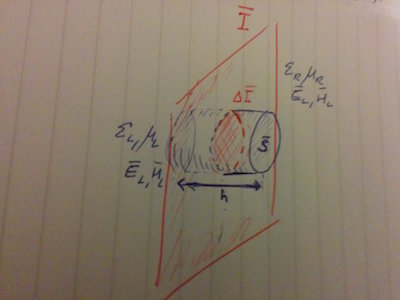
\includegraphics[scale=]{Figures/Chapters/PhysicalProblem/interfaceEPillBox}
\end{center}
\caption{}
\label{fig:material-interface-derivation:E-pillbox}
\end{figure}

In the limit $h \to 0$ all electric flux leaves the volume through the parallel planes of the surface $S$, and \eqref{maxwell-gauss-integral} can be written as

$$
\mathbf{D}_L \cdot \hat{\mathbf{n}} \Delta A  - \mathbf{D}_R \cdot \hat{\mathbf{n}} \Delta A = \rho_s \Delta A
$$

where we have assumed that $S$ is sufficiently small that $D$ may be considered constant. The material interface condition can be written as

$$
\mathbf{D}_L \cdot \hat{\mathbf{n}} - \mathbf{D}_R \cdot \hat{\mathbf{n}} = \rho_s
$$

Note that in the case where $\rho_s = 0$, that is there are no free (unbound) charges then the normal component of the electric flux density, $D$, is continuous across the interface.

By following the analogous procedure for the magnetic field using \eqref{maxwell-gauss-magnetism-integral} we obtain that

$$
\mathbf{B}_L \cdot \hat{\mathbf{n}} = \mathbf{B}_R \cdot \hat{\mathbf{n}}
$$

These conditions are used with maxwells divergence equations.
% not used in the code!?

\subsubsection{Tangental Fields}

Similarily for the tangental component of electric field we consider a closed rectangular integration path in the plane of $E_L$ and $E_R$ around the same interface shown in \ref{fig:material-interface-derivation:E-schematic}, as shown in \ref{fig:material-interface-derivation:E-rectangular-loop}. Again in the limit $h \to 0$ and noting that $d\mathbf{S} = 0$ we can write \eqref{eq:maxwell-faraday-integral} as

\begin{equation}
\label{eq:material-interfaces-tangentalcondition-E}
\int_{L_1}^{L_2} \mathbf{E}_L \cdot d\mathbf{l} - \int_{R_1}^{R_2} \mathbf{E}_R \cdot d \mathbf{l} = 0
\end{equation}

or

$$
\mathbf{E}_L \cdot d\mathbf{l} = \mathbf{E}_R \cdot d \mathbf{l}
$$

The resulting interface condition is therefore that components of $\mathbf{E}$ tangiental to the interface are continuous - which can be written more generally as

$$
\hat{\mathbf{n}} \times \mathbf{E}_L = \hat{\mathbf{n}} \times \mathbf{E}_R 
$$

Again following an analogous for magnetic field we obtain

$$
\hat{\mathbf{n}} \cdot \mathbf{H}_L = \hat{\mathbf{n}} \times \mathbf{H}_R
$$

These conditions are used with maxwells curl equations.

\subsubsection{PEC}

Metals with a large number of conduction band electrons are well approximated by the perfect electric conduction (PEC) approximation. In a PEC the coulomb repulsion between electrons is assumed to cause all free charges to be distributed in an infinitesimally thin layer on the surface of the material. Since free charge exists within the material and the change distribution instantaneously to counteract any applied electric fields. Let us consider that the material on the right hand side of the interface described above is a PEC. In this case, since $E_R$ is zero inside the material then equation \eqref{eq:material-interfaces-tangentalcondition-E} becomes simply

$$
\int_{L_1}^{L_2} \mathbf{E}_L \cdot d\mathbf{l} - \int_{R_1}^{R_2} \mathbf{E}_R \cdot d \mathbf{l} = 0
$$

and the resulting condition is

$$
\mathbf{E}_L \times \hat{\mathbf{n}} = 0
$$

and similarily for the magnetic field

$$
\mathbf{H}_L \times \hat{\mathbf{n}} = \mathbf{J}_s
$$

% what about the other two conditions i.e. divergence conditions - should I specify those too?
where $\mathbf{J}_s$ is the surface current.

\subsection{Silver-Muller radiation condition}

\section{Reduction to 2 dimensions}

\subsection{TE and TM modes}
For a physical system where the electric field is invariant to one of the cartesian variables then the derivatives with respect that variables become zero and Maxwells equations are decoupled into two sets of coupled equations with three unknowns each. By convention we choose the z coordinate as the direction of invariance and the resulting modes are known as the $TE_z$ and $TM_z$ modes. The $TE_z$ modes is given by

\begin{equation*}
\begin{array}{ccccc}
\mathbf{U}_1 = \begin{pmatrix} \epsilon E_1 \\ \epsilon E_2 \\ \mu H_3 \\ J_1 \\  J_2 \end{pmatrix} ,
&
\mathbf{F}_1 = \begin{pmatrix} 0 \\ H_3 \\ E_2 \\ 0 \\  0 \end{pmatrix} ,
&
\mathbf{F}_2 = \begin{pmatrix} - H_3 \\ 0 \\ -E_1 \\ 0 \\ 0 \end{pmatrix} ,
&
\mathbf{S} = \begin{pmatrix} - J_1 \\ - J_2 \\ 0 \\ \omega^2 \, E_1 - \gamma J_1 \\  \omega^2 \, E_2 - \gamma J_2 \end{pmatrix} ,
\end{array}
\:
\end{equation*}

and the $TM_z$ mode is

\begin{equation*}
\begin{array}{ccccc}
\mathbf{U}_1 = \begin{pmatrix} \epsilon E_3 \\ \mu H_1 \\ \mu H_2 \\ J_3 \end{pmatrix} ,
&
\mathbf{F}_1 = \begin{pmatrix} -H_2 \\ 0 \\ -E_3 \\ 0 \end{pmatrix} ,
&
\mathbf{F}_2 = \begin{pmatrix} H_1 \\ E_3 \\ 0 \\ 0 \end{pmatrix} ,
&
\mathbf{S} = \begin{pmatrix} - J_3 \\ 0 \\ 0 \\ \omega^2 \, E_3 - \gamma J_3 \end{pmatrix} ,
\end{array}
\:
\end{equation*}
.

In practice a number of real systems, notably systems which can be approximated as having infinite extent in one direction, can be by approximated by an invariant electric field in one direction.

\subsection{2D Compact Form}

Several physical systems, notably wave guides, may have known modal dependence in a given direction. Let us assume that the z-dependence of all electromagnetic fields of a system is known to vary with z as:

\begin{equation}
    E_z = \tilde{E}_z e^{-i \beta_z z}
    H_z = \tilde{H}_z e^{-i \beta_z z}
\label{compact2D-zdep}
\end{equation}

By substituting \ref{compact2D-zdep} into \ref{maxwell-curl-equations-conservation-form} we obtain in the compact form of Maxwells equations [***ref]

*** ....

Note that when $\beta_z = 0$ this decouples into the $TE_z$ and $TM_z$ modes as expected since in this case there is no dependence on z-dependence.

\begin{itemize}
  \item Mention beta for z-dependence
  \item Obtain formulation from 3D. Mention B=0 -> equations decouple into TE/TM mode
\end{itemize}

\section{Relation to Wave Equation and Helmholtz Equation}
\begin{itemize}
  \item discuss Freq vs Time domain - broadband response
  \item justify TD
  % conclude why, never touch again.
\end{itemize}

\subsection{Wave Equation}

Consider the maxwell curl equations for free space for simplicity, and rewriting in terms of $B$ and $E$ using the constitutive equations \ref{contitutive-linear-non-dispersive-1} and \ref{contitutive-linear-non-dispersive-2} rewritten here for convenience

\begin{equation}
 \nabla \times \mathbf{B} = \frac{\partial \epsilon_0 \mathbf{E}}{\partial t}
 \label{maxwell-curl-B-free-space}
\end{equation}.
\begin{equation}
 \nabla \times \mathbf{E} = - \frac{\partial \mathbf{B}}{\partial t}
\end{equation}.

Taking the curl of each equation and subsituting from \ref{maxwell-gauss-1} and \ref{maxwell-gauss-2} we obtain:

\begin{equation}
    \nabla \times ( \nabla \times \mathbf{B} ) = \frac{\partial \epsilon_0 ( \nabla \times \mathbf{E} ) }{\partial t}
    \label{maxwell-curl-curl-B}
\end{equation}.
\begin{equation}
 \nabla \times \mathbf{E} = - \frac{\partial \mathbf{B}}{\partial t}
    \label{maxwell-curl-curl-E}
\end{equation}.

By using the vector identity

$$
\nabla \times ( \nabla \times \mathbf{V} ) = \nabla \cdot ( \nabla \cdot \mathbf{V} ) - \nabla^2 \mathbf{V}
$$,

noting that from Maxwells equations $\nabla \cdot \mathbf{V} = 0$ for both $\mathbf{V} = \mathbf{E}$ and $\mathbf{V} = \mathbf{B}$

and using \eqref{maxwell-curl-B-free-space} we can rewrite \eqref{maxwell-curl-curl-B} and \eqref{maxwell-curl-curl-E} as

$$
\nabla^2 \times \mathbf{E} - c \frac{\partial}{\partial t} \mathbf{E} = 0
$$

$$
\nabla^2 \times \mathbf{B} - c \frac{\partial}{\partial t} \mathbf{B} = 0
$$

or in vector form as

\begin{equation}
\nabla^2 \times \mathbf{U} = c \frac{\partial}{\partial t} \mathbf{U} = 0
\label{maxwell-wave-eqtn}
\end{equation}

which is Maxwells equations in wave equation form. The same treatment can be made easily extended to waves in a dielectic medium.

\subsection{Helmholtz Equation}
If we assume that all components of an electromagnetic wave are separable as
$$
\mathbf{U}(\mathbf{x},t) = \mathbf{X}(\mathbf{x}) T(t)
$$
where $\mathbf{X}$ is an envelope which modulates the amplitude of a known time dependence, given by $T$ then \ref{maxwell-wave-eqtn} can be written as

$$
\frac{\nabla^2 \times \mathbf{X}}{\mathbf{X}} = c \frac{1}{T} \frac{\partial T}{\partial t }
$$

By employing separation of variable, with a seperation variable $-k^2$ we obtain a partial differential equation in time

\begin{equation}
\nabla^2 \times \mathbf{X} + k^2 \mathbf{X} = 0
\label{eq-helmholz-time}
\end{equation}

and an ordinary differential equation in time

\begin{equation}
\frac{\partial T}{\partial t} + \omega ^2 T  = 0
\label{eq-helmholz-time}
\end{equation}

where we define $\omega = k c$.

The general solution to \eqref{eq-helmholz-time} is of the form
$$
T(t) = \sum A e^{i \omega t}
$$

For a system with a single angular frequency $\omega_f$ the complete solution to the system of equations can be obtained by solving \eqref{eq-helmholz-time} and employing the ***. This is the basis of frequency-domain approaches, however solving Maxwells equations in this way involves running a single finite element simulation for each value of $\omega$ of interest. This illustrates the key advantage of time domain approaches, namely the ability to capture the broadband frequency response of a system in a single run of the simulation.


